
F�r den USB Gadget Modus der Raspberry Pi Zero wird bereits eine vorkonfigurierte MicroSD-Karte bzw. ein MicroSD-Karten-Image zur Verf�gung gestellt. Darauf sind bereits alle Voreinstellungen getroffen worden sodass nur eine minimale Anpassung erfolgen muss. Sollte die Einrichtung manuell erfolgen so muss man sich das PDF-Dokument 'Raspberry Pi Jam - Raspjamming Admin' besorgen. 

\subsection{Host (DHCP-Client)}
%\clearpage
\subsubsection{Kubuntu 16.04}

Am Host-PC muss bei den IPv4-Einstellungen die Methode "`Automatisch"' eingestellt sein. Wenn es sich um eine neue Verbindung handelt, ist dies bereits voreingestellt, eine Parametrierung kann dann entfallen. Ansonsten muss zur Konfiguration unter Linux (Kubuntu 16.04) zuerst der Dialog "`Netzwerkverbindungen"' ge�ffnet werden.\\ 
Dazu klickt man mit der rechten Maustaste auf das Netzwerksymbol in Infobereich rechts unten. Dann kann die Option "`Netzwerkverbindungen einrichten..."' ausgew�hlt werden.

\begin{figure}[ht]
  \centering
  
\includegraphics[scale=1.00]{images/OTG_NetzwerkverbindungenIcon.png}	
  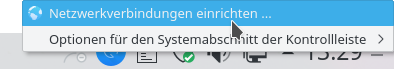
\includegraphics[scale=0.42]{images/OTG_NetzwerkverbindungenOpen.png}	
  %	\caption{}
  \label{OTG_LINUX_NetzwerkverbindungenApp}
\end{figure}


Nun k�nnte die neue "`Kabelnetzwerkverbindung"' umbenannt werden, z.~B. in Raspberry Pi Zero. Erkennen kann man das Netzwerk an der Mac-Adresse, die man bei "`g\_ether.host\_addr"' angegeben hat (z.~B. 00:01:02:03:04:05).  


\begin{figure}[ht]
  \centering
  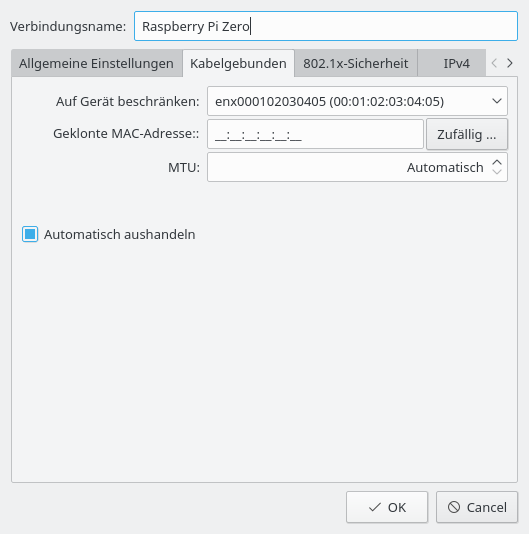
\includegraphics[scale=0.42]{images/OTG_Pi_Verbindungsname.png}
	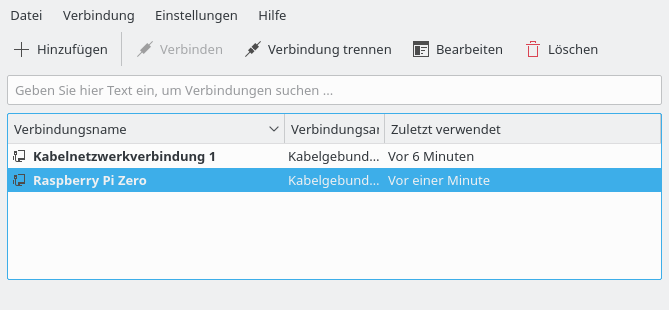
\includegraphics[scale=0.42]{images/OTG_Netzwerkverbindungen.png}
%	\caption{}
  \label{OTG_LINUX_Netzwerkverbindungen}
\end{figure}


Nun kann bei den IPv4-Einstellungen die Methode "`Automatisch"' eingestellt werden.

%\begin{figure}[ht]
%  \centering
%  \includegraphics[scale=0.42]{images/OTG_NetzwerkverbindungenAutomatisch.png}
%	\caption{}
%  \label{OTG_LINUX_Netzwerkverbindungen}
%\end{figure}

%\clearpage
%\input{OTG_Mint}

%\subsection{Internet Zugriff} 
~\\
Nach der Einrichtung des Netzwerk kann der Raspberry Pi Zero mit dem Namen "`raspberrypi.local"' erreicht werden. Um den Raspbery Pi Zero mit dem Internet verbinden zu k�nnen m�ssen einige Einstellungen am Host %und Client
 gemacht werden. Man muss den Name des Netzwerkger�ts am Host-PC kennen, das mit dem Internet verbunden ist. Dies ermittelt man �ber die Netzwerkeinstellungen oder �ber die Konsole mit nmcli. Im Beispielfall ist der Name "`enp0s25"' das richtige Ger�t.

\begin{console} 
	nmcli d
\end{console} 

\begin{screensmall} 
	GER�T            TYP       STATUS           VERBINDUNG        
	enx000102030405  ethernet  verbunden        Raspberry Pi Zero 
	enp0s25          ethernet  verbunden        Netzwerkverbindung 1                
	lo               loopback  nicht verwaltet  --  
\end{screensmall}

Damit der Internetzugang f�r den Raspberry Pi Zero freigegeben wird, m�ssen am Host-PC folgende Befehle in einem Terminal eingeben werden. "`enp0s25"' muss durch den Namen des Netzwerkger�ts ersetzt werden, das mit dem Internet verbunden ist.

\begin{console} 
	sudo sysctl -w net.ipv4.ip_forward=1
	sudo iptables -t nat -A POSTROUTING -o enp0s25 -j MASQUERADE
\end{console}



Alternativ k�nnen die Einstellungen auch automatisch �ber eine Shell-Script durchgef�hrt werden (siehe Kapitel \ref{sec:shellscript} \titleref{sec:shellscript}).


\section{Verbindung}

\subsection{SSH}

Nach der Einrichtung kann per SSH-Client eine Verbindungen zum Raspberry Pi hergestellt werden. Dazu muss in einem Terminal folgender Befehl eingegeben werden:

\begin{console} 
	ssh -X pi@raspberrypi.local
\end{console}

Um grafische Programme am Host anzeigen zu k�nnen, muss der Parameter \texttt{-X} angegeben werden. "`\textbf{pi}"' ist der Standardbenutzer am System. Dann wird eine X-Server Verbindung via SSH hergestellt. Verbindet man sich zum ersten Mal mit dem Raspberry Pi, so wird noch eine Sicherheitswarnung ausgegeben. Der kryptographische Schl�ssel f�r die Verbindung ist dem lokalen System noch nicht bekannt.%  und muss best�tigt werden.
\begin{screensmall}
The authenticity of host 'raspberrypi.local (192.168.137.10)' can't be established.
ECDSA key fingerprint is SHA256:Dcf3HYgE2GHnNnZ8Xhv8iJ9yA+zvfXBC9COm2eL9i0w.
Are you sure you want to continue connecting (yes/no)? 
Warning: Permanently added 'raspberrypi.local,192.168.137.10' (ECDSA) to the list of known hosts.
\end{screensmall}

Die Frage muss mit \texttt{yes} best�tigt werden. Anschlie�end muss das Default-Passwort von Raspbian "`\textbf{raspberry}"' eingegeben werden. Nun sollte man den Raspberry Pi Prompt \texttt{pi@rasbperrypi:\textasciitilde  \$} sehen. 

Wechselt man zu einem anderen Raspberry Pi mit den gleichen Namen oder installiert das System nochmals, so kann es passieren, dass eine Fehlermeldung ausgegeben wird, weil sich der kryptographische Schl�ssel ge�ndert hat.

\begin{screensmall} 
@@@@@@@@@@@@@@@@@@@@@@@@@@@@@@@@@@@@@@@@@@@@@@@@@@@@@@@@@@@
@    WARNING: REMOTE HOST IDENTIFICATION HAS CHANGED!     @
@@@@@@@@@@@@@@@@@@@@@@@@@@@@@@@@@@@@@@@@@@@@@@@@@@@@@@@@@@@
\end{screensmall} 

%The ECDSA host key for raspberrypi.local has changed,
%and the key for the corresponding IP address 169.254.229.192
%is unknown. This could either mean that
%DNS SPOOFING is happening or the IP address for the host
%and its host key have changed at the same time.
%@@@@@@@@@@@@@@@@@@@@@@@@@@@@@@@@@@@@@@@@@@@@@@@@@@@@@@@@@@@
%@    WARNING: REMOTE HOST IDENTIFICATION HAS CHANGED!     @
%@@@@@@@@@@@@@@@@@@@@@@@@@@@@@@@@@@@@@@@@@@@@@@@@@@@@@@@@@@@
%IT IS POSSIBLE THAT SOMEONE IS DOING SOMETHING NASTY!
%Someone could be eavesdropping on you right now (man-in-the-middle attack)!
%It is also possible that a host key has just been changed.
%The fingerprint for the ECDSA key sent by the remote host is
%SHA256:Dcf2HYyE2GHnNpZ8Xhv8iJ9yj+zvfXBC9COm2eL9i0w.
%Please contact your system administrator.
%Add correct host key in /home/evil/.ssh/known_hosts to get rid of this message.
%Offending ECDSA key in /home/evil/.ssh/known_hosts:9
%remove with:
%ssh-keygen -f "/home/evil/.ssh/known_hosts" -R raspberrypi.local
%ECDSA host key for raspberrypi.local has changed and you have requested strict checking.

In diesem Fall muss man die Verbindung aus den bekannten Hosts l�schen. Hierf�r muss folgendes Kommando ausgef�hrt werden:

\begin{console} 
	ssh-keygen -R raspberrypi.local
\end{console}

Optional kann auch der Parameter \texttt{-o UserKnownHostsFile=/dev/null} beim ssh-Befehl hinzugef�gt werden. Dann erfolgt keine �berpr�fung der Verbindung. 


\subsection{SSH �ber Shell-Script} \label{sec:shellscript}

Das Einfachste ist die Verbindung zu Raspberry Pi �ber das vorbereitete PiConnect.sh Shell-Script herzustellen. Es setzt automatisch die Internetweiterleitung und startet die SSH-Verbindung. Es kann vom vorbereitetet Raspbian Image oder von Github geladen werden.

\begin{console} 
	scp pi@raspberrypi.local:/home/pi/scripts/PiConnect.sh .
\end{console}
oder
\begin{console} 
	wget --trust-server-names https://goo.gl/uwguQo
	sh PiConnect.sh
\end{console}   


